\documentclass{beamer}
 
\usepackage[utf8]{inputenc}
\usepackage{amsmath}
\usepackage{clrscode3e}
\usepackage{graphicx}
\usepackage{tikz}
\usetikzlibrary{arrows}
\usetikzlibrary{backgrounds}

\graphicspath{{imgs/}}


%Information to be included in the title page:
\title{Semi-supervised Learning with Deep Generative Models}
\subtitle{Kingma et. al. (2014)}
\author{Tyler Brown}
\institute{CS 7180}
\date{}
 
\begin{document}
 
\frame{\titlepage}
 
\begin{frame}
  \frametitle{Motivating Question}
  How can we model data of increasing size when obtaining label 
  information is difficult?
\end{frame}

\begin{frame}
  \frametitle{High-level Answer}

  We can estimate missing label information by
  using a probabilistic model.
  
\end{frame}

\begin{frame}
  \frametitle{Most Relevant Previous Work}

  Pitelis, N., Russell, C., and Agapito, L. (2014). Semi-supervised
  learning using an unsupervised atlas. \textit{In Proceddings of the
    European Conference on Machine Learning (ECML)}, volume LNCS 8725,
  pages 565 – 580.

  \begin{itemize}
  \item Observing that high-dimensional datasets often lie on or near
    \textit{manifolds} of locally low rank can help avoid the
    \textit{curse of dimensionality}
  \item Experiments show how using unlabelled data to learn the underlying
    manifold improves classifier accuracy when trained on limited labelled
    data
    \begin{enumerate}
    \item \textbf{Unsupervised learning of the underlying manifold:}
      Approximate the manifold of data on the original space by fitting
      an atlas of low-dimensional overlapping affine charts.
    \item \textbf{Supervised training of an SVM:} Proposed a new family of
      Mercer Kernels for SVM-based supervised learning which uses
      soft-assignment of datapoints to the underlying low-dimensional affine
      charts to generate the kernels
      \end{enumerate}
    \end{itemize}

  \end{frame}

\begin{frame}
  \frametitle{Specifying the Probabilistic Model for Missing Labels}

  Kingma et. al. (2014)
  
    \begin{itemize}
  \item Data appears as pairs $(\mathbf{X}, \mathbf{Y}) =
    \{(\mathbf{x}_1, y_1), ..., (\mathbf{x}_N, y_N)\}$
  with the $i$-th observation $x_i \in \mathbb{R}^D$ and a
  corresponding class label $y_i \in \{1, ..., L\}$

  \begin{itemize}
\item Each pair of observations $(x_i,y_i)$ has a corresponding
  latent variable $z_i$

\item Empirical distribution over the labelled and unabelled subsets
  is referred to as $\tilde{p_l}(\mathbf{x}, y)$ and
  $\tilde{p_u}(\mathbf{x})$
  \end{itemize}
\item We can estimate $y_i$ for $x_i$ in distribution
  $\tilde{p_u}(\mathbf{x})$ by finding the maximum
  probability of $p(y_i)$ by using a set of features
  related to $z_i$ and a predictive model
  \begin{enumerate}
  \item \textbf{Latent-feature discriminative model (M1)}
  \item \textbf{Generative semi-supervised model (M2)}
  \item \textbf{Stacked generative semi-supervised model (M1+M2)}
  \end{enumerate}
  \end{itemize}
  \end{frame}

\begin{frame}
  \frametitle{Bayes Rule is used when specifying M1 \& M2}

  \begin{align*}
    p(x,y) &= p(x)p(y|x) \\
    &= p(y)p(x|y) \\
    p(x|y) &= \frac{p(x)p(y|x)}{p(y)}
  \end{align*}

  for models M1 \footnotemark, $p(z|x)$, and M2 \footnotemark; $p(y|x)$

  \footnotetext[1]{Kingma et. al. (2014) equation (1)}
  \footnotetext[2]{Kingma et. al. (2014) equation (2)}
  
\end{frame}

\begin{frame}
  \frametitle{(M1) Latent-feature discriminative model}

  \[
  y \Leftarrow   p(z|x) = \frac{p(z)p(x|z)}{p(x)}
  \]

  where

  \begin{align*}
    p(z) &= \mathcal{N}(z|0,I) \qquad \text{Gaussian distribution of $z$ given a missing label $y$}\\
    p(x|z) &= f(x;z,\theta) \qquad \text{likelihood function, parameters
      $\theta$ of a set of $z$} \\
    p(x) &= \tilde{p_u}(x) \qquad \text{unlabelled subset of $x_i \in \mathbb{R}^D$}
    \end{align*}

  Kingma et. al. (2014) eq. (1)
\end{frame}

\begin{frame}
  \frametitle{(M1) Predicting Class Labels $y$}

  Approximate samples from the posterior distribution over the
  latent variables $p(z|x)$ are used as features to train a
  classifier that predicts class labels $y$

  \begin{center}
    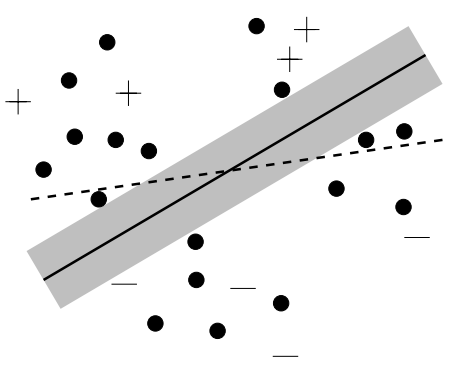
\includegraphics[scale=0.5]{fig6_2}
  \end{center}

  (transductive) SVM\footnotemark finds the largest margin w.r.t.
  the training \underline{\textbf{and}} the test vectors


  \footnotetext{See Figure 6.2 from Chapelle, O., B. Schölkopf,
    and A. Zien. "Semi-Supervised Learning." (2006).}
\end{frame}

\begin{frame}
  \frametitle{(M2) Generative semi-supervised model}

  \[
  p(y|\mathbf{x}) = \frac{p(\mathbf{x}|y) p(y)}{p(\mathbf{x})} \approx
  \frac{p_\theta (\mathbf{x}|y, \mathbf{z}) p(y)}{p(\mathbf{x})}
  \]

  where

  \begin{align*}
    p(y) &= Cat(y|\mathbf{\pi}) \qquad \text{multinomial distribution, $y$ can be latent} \\
    p(\mathbf{z}) &= \mathcal{N}(\mathbf{z|0,I}) \qquad
    \text{Gaussian distribution of $z$ when missing $y$} \\
    p_\theta (\mathbf{x}|y,z) &= f(\mathbf{x};y,\mathbf{z},\mathbf{\theta})
    \qquad \text{likelihood function, nonlinear parameters} \\
    p(x) & \qquad \qquad \qquad \qquad \text{all $x$ in dist. of real numbers;  $x \in \mathbb{R}^{D}$}
    \end{align*}
  
\end{frame}

\begin{frame}
  \frametitle{Stacked generative semi-supervised model (M1 + M2)}

  Combine M1 and M2
  \begin{enumerate}
  \item Learn a new latent representation $z_1$ from M1
  \item Use embeddings from $z_1$ instead of raw data $x$, to create
    a generative semi-supervised model M2
  \end{enumerate}

  \begin{center}
  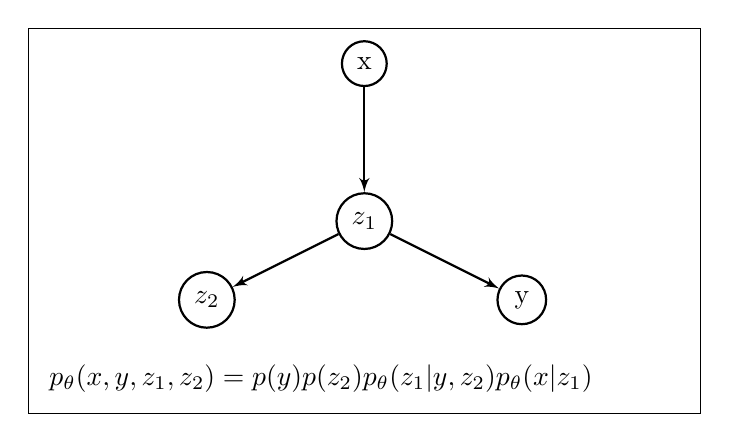
\begin{tikzpicture}[scale=1, thick, framed,background rectangle]
    \tikzset{vertex/.style = {shape=circle,draw,minimum size=1.5em}}
    \tikzset{edge/.style = {->,> = latex'}}

    % vertices
    \node[vertex] (x) at (4,3) {x};
    \node[vertex] (z1) at (4,1) {$z_1$};
    \node[vertex] (z2) at (2,0) {$z_2$};
    \node[vertex] (y) at (6,0) {y};
    \node[text width=8cm] (t) at (4,-1) {
      $p_\theta (x,y,z_1,z_2) = p(y)p(z_2)p_\theta
      (z_1|y,z_2)p_\theta(x|z_1)$};

    % edges
    \draw[edge] (x) to (z1);
    \draw[edge] (z1) to (z2);
    \draw[edge] (z1) to (y);
  \end{tikzpicture}
  \end{center}

  

\end{frame}

\begin{frame}
  \frametitle{Scaling Up: Lower Bound Objective}

  Lower Bound Objective\footnotemark: computation of the exact posterior
  distribution is intractable for models M1 and M2
  
  \begin{align*}
    \text{M1: } &q_\phi (z|x) = \mathcal{N}(z|u_\phi (x),
    \text{diag}(\mathbf{\sigma}_\phi^2 (\mathbf{x}))) \tag{3}\\
    \text{M2: } &q_\phi(\mathbf{z}|y,\mathbf{x}) =
    \mathcal{N}(\mathbf{z}|\mathbf{\mu}_\phi (y, \mathbf{x}),
    \text{diag}(\mathbf{\sigma}_\phi^2(\mathbf{x}))); \\
    &q_\phi (y|\mathbf{z}) = \text{Cat}(y|\mathbf{\pi}_\phi (x)), \tag{4}
  \end{align*}

  where

  \begin{align*}
    \sigma_\phi (x) &\qquad \text{vector of standard deviations} \\
    \pi_\phi(x) &\qquad \text{probability vector} \\
    \mu_\phi(x), \sigma_\phi(x), \pi_\sigma (x)  &\qquad
    \text{Maximum likelihood Priors (MLPs)} \\
    \end{align*}

  \footnotetext{Kingma et. al. (2014) equations (3), (4)}
\end{frame}

\begin{frame}
  \frametitle{Scaling Up: M1 Model Objective}

  Variational bound $\mathcal{J}(x)$ on the marginal likelihood of
  a single data point is\footnotemark
  \[
  \log p_\theta (x) \ge \mathbb{E}_{q_\phi (z|x)}
       [\log p_\theta (x|z)] - KL[q_\phi (z|x)||p_\theta (z)]
       = - \mathcal{J}(x)
   \]

   Approximate posterior is used as a feature extractor for the
   labelled data set, and the features used for training the
   classifier

  \footnotetext{Kingma et. al. (2014) Equation 5}
\end{frame}

\begin{frame}
  \frametitle{Scaling Up: M2 Model Objective}

  When $y_i$ is observed for the $(x_i,y_i)$ data pair, extend from M1
  \begin{align*}
    &\log p_\theta (x) \ge \mathbb{E}_{q_\phi (z|x,y)}
       [\log p_\theta (x|y,z) + \log p_\theta (y) + \log p(z) -
         q_\theta (z|x,y)] \\
       &= - \mathcal{L}(x,y)
  \end{align*}

  In the case where $y_i$ is missing,
  \begin{align*}
    \log p_\theta (x) &\ge \mathbb{E}_{q_\phi (y,z|x)}
         [\log p_\theta (x|y,z) + \log p_\theta (y) \\
           &\qquad\qquad\qquad + \log p(z) - \log q_\phi (y,z|x)] \\
         &= \sum_y q_\phi (y|x) ( - \mathcal{L}(x,y))
         + \mathcal{H}(q_\phi (y|x)) \\
         &= - \mathcal{U}(x)
  \end{align*}

  The bound on the marginal likelihood for the entire dataset is
  now\footnotemark
  \[
  \mathcal{J} = \sum_{(x,y) \sim \tilde{p}_l} \mathcal{L}(x,y)
    + \sum_{x \sim \tilde{p}_u} \mathcal{U}(x)
    \]

    \footnotetext{See Kingma et. al. (2014) equations 6-9}
\end{frame}

\begin{frame}
  \frametitle{Optimization Techniques}

  \begin{itemize}
  \item Bounds from M1 and M2 objective function equations provides
    for optimization of both $\theta$ and $\phi$ parameters
    \begin{itemize}
    \item Optimization can be done \textit{jointly} without using the EM
      Algorithm
    \end{itemize}
  \item Use deterministic reparameterizations of the expectations in
    the objective function and \textit{Monte Carlo} approximation
  \item Previous work refers to this as \textit{stochastic gradient
    variational Bayes}\footnotemark and
    \textit{stochastic backpropagation}\footnotemark
  \end{itemize}

  \footnotetext[7]{Kingma, D. P. and Welling, M. (2014).
    Auto-encoding variational Bayes. \textit{In Proceedings of the
      International Conference on Learning Representations (ICLR)}.}
  \footnotetext{Rezende, D. J., Mohamed, S., and Wierstra, D. (2014).
    Stochastic backpropagation and approximate inference
    in deep generative models. \textit{In Proceedings of the International
      Conference on Machine Learning (ICML)}, volume 32 of JMLR W&CP.}

\end{frame}

\begin{frame}
  \frametitle{Optimization Algorithms}
  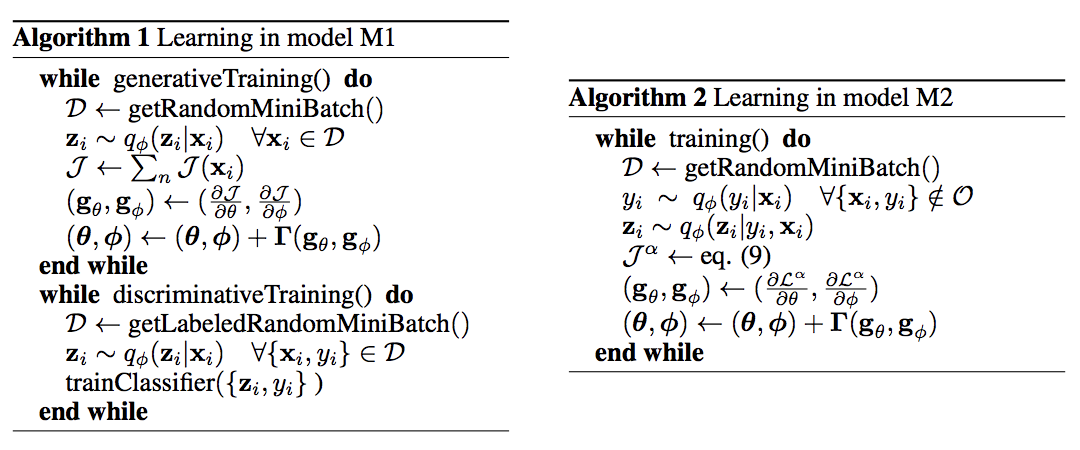
\includegraphics[scale=0.5]{learningModel}

  Gradients w.r.t. generative parameters $\theta$ and variational
  parameters $\phi$ can be efficiently computed as expectations of
  simple gradients\footnotemark

    \[
  \nabla_{\{\theta, \phi\}} \mathbb{E}_{q_\phi (z|x)}
        [\log p_\theta (x|z)] = \mathbb{E}_{\mathcal{N}(\epsilon | 0, I)}
        [\nabla_{\{\theta, \phi\}} \log p_\theta (x |\mu_\theta (x)
          + \sigma_\phi (x) \odot \epsilon)]. 
        \]

  \footnotetext{Kingma et. al. (2014) equation 11, regarding M1}
\end{frame}

\begin{frame}
  \frametitle{Results: Benchmark Classification}

  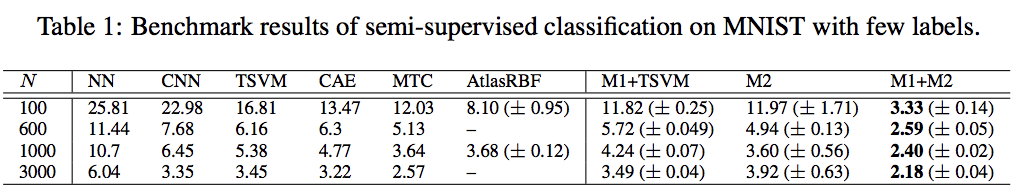
\includegraphics[scale=0.5]{table1}

  \begin{itemize}
  \item Varying the size of labelled data from 100 to 3000
  \item SoftPlus Activation function
    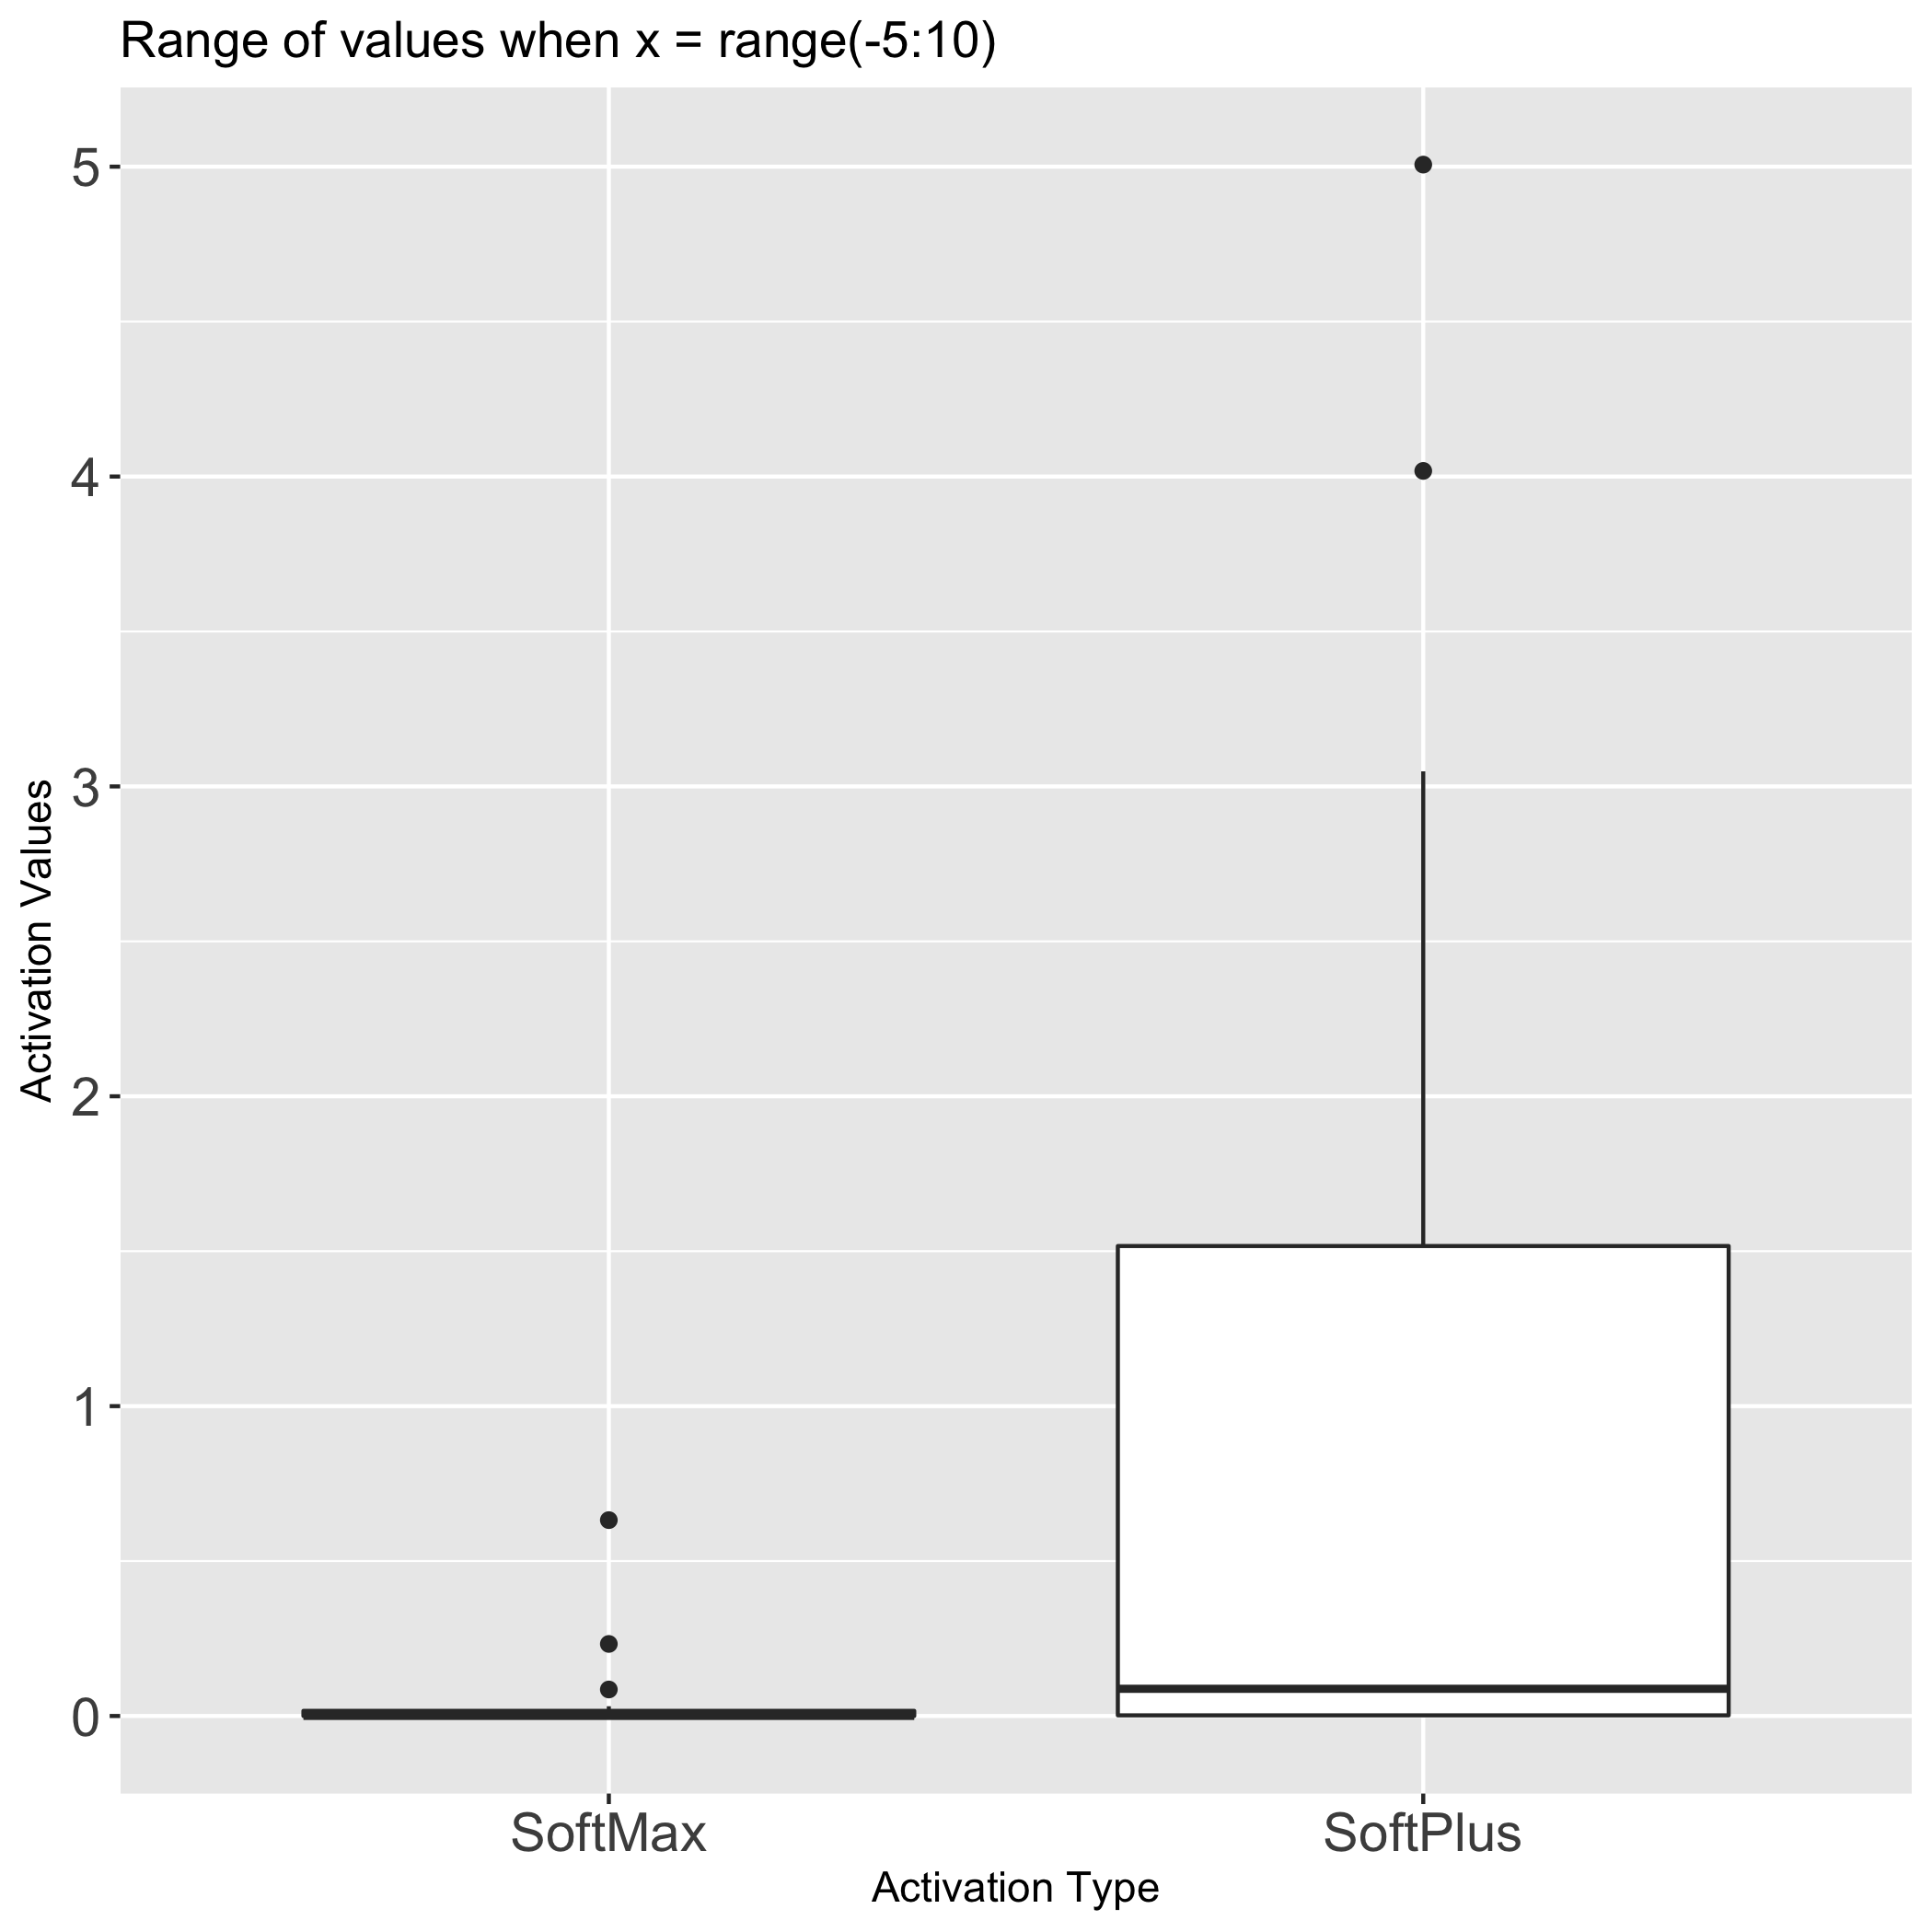
\includegraphics[scale=0.05]{activations}
    \end{itemize}
  
\end{frame}
\begin{frame}
  \frametitle{Results: Image Classification}

  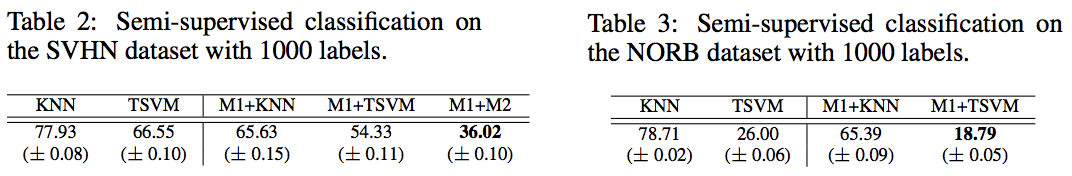
\includegraphics[scale=0.5]{table2and3}

  \begin{itemize}
  \item No comparative results in semi-supervised setting exists for
    SVHN and NORB image data sets
  \item Performed nearest-neighbor and TSVM classification with RBF
    kernels
  \item Compared performance on features generated by their latent-feature
    discriminative model to the original features
    \end{itemize}

\end{frame}

\begin{frame}
  \frametitle{Discussion}

  You can use this model for a few things

  TODO: just summarize their discussion
\end{frame}

\begin{frame}
  \textbf{Any questions? Thanks!}
  \end{frame}


 
\end{document}
